\documentclass[12pt,a4paper]{article}
\usepackage[utf8]{inputenc}
\usepackage[margin=1in]{geometry}
\usepackage{amsmath}
\usepackage{amsfonts}
\usepackage{amssymb}
\usepackage{graphicx}
\usepackage{listings}
\usepackage{xcolor}
\usepackage{fancyhdr}
\usepackage{titlesec}
\usepackage{tikz}
\usepackage{enumerate}
\usetikzlibrary{positioning,shapes,arrows}
\usepackage[colorlinks=true, linkcolor=blue, urlcolor=blue, citecolor=blue]{hyperref}

% SQL syntax highlighting
\lstdefinestyle{sqlstyle}{
    language=SQL,
    basicstyle=\ttfamily\small,
    keywordstyle=\color{blue}\bfseries,
    commentstyle=\color{green!50!black},
    stringstyle=\color{red},
    numbers=left,
    numberstyle=\tiny\color{gray},
    numbersep=5pt,
    breaklines=true,
    breakatwhitespace=true,
    tabsize=2,
    showspaces=false,
    showstringspaces=false,
    frame=single,
    rulecolor=\color{gray!30},
    backgroundcolor=\color{gray!5}
}

\lstset{style=sqlstyle}

% Page setup
\pagestyle{fancy}
\fancyhf{}
\rhead{CSE 414 - Task 3}
\lhead{Database Normalization Analysis}
\cfoot{\thepage}

% Title formatting
\titleformat{\section}{\Large\bfseries}{}{0em}{}
\titleformat{\subsection}{\large\bfseries}{}{0em}{}

\begin{document}

% Title Page
\begin{titlepage}
    \begin{figure}[htbp]
    \centering
    
\includegraphics[width=0.2\textwidth]{cu.png}
    \end{figure}
    \centering
    \vspace*{0.5cm}
    {\Huge\bfseries University of Chittagong}\\[0.5cm]
    {\Large Department of Computer Science \& Engineering}\\[0.5cm]
    {\large Database Systems Lab}\\[2cm]
    
    {\large Name of the assignment:}\\[0.3cm]
    {\LARGE\bfseries Task 3: Refinement, Normalization, and SQL-DDL\\[0.5cm]}
    {\large CSE 414}\\[0.5cm]
    {\large Medical Database Analysis}\\[3cm]
    
    \begin{minipage}[t]{0.4\textwidth}
    \raggedleft
    Submitted By:\\
    \large \textbf{Debashish Chakraborty}\\
    \large ID: 23701034
    \end{minipage}
    \hspace{0.05\textwidth}
    \vrule width 1pt
    \hspace{0.05\textwidth}
    \begin{minipage}[t]{0.4\textwidth}
    Submitted To:\\
    \large \textbf{Dr. Rudra Pratap Deb Nath}\\
    \large Associate Professor
    \end{minipage}
    
    \vfill
    {\large July 6, 2025}
\end{titlepage}

\newpage
\tableofcontents
\newpage 

\section{Introduction}

This report analyzes the medical database schema created in previous tasks, focusing on functional dependencies, normalization theory, and the application of normal forms.

\section{Current Database Schema}

The current normalized schema consists of the following relations:

\begin{enumerate}
    \item \textbf{Drug}(drug\_name, drug\_category, product\_name, company\_name)
    \item \textbf{SideEffect}(name)
    \item \textbf{Disease}(disease\_name, disease\_category)
    \item \textbf{ClinicalTrial}(clinical\_trial\_title, clinical\_trial\_start\_date, clinical\_trial\_completion\_date, clinical\_trial\_participants, clinical\_trial\_status, clinical\_trial\_address, clinical\_trial\_institution, clinical\_trial\_address\_1, clinical\_trial\_main\_researcher)
    \item \textbf{ClinicalTrialCondition}(name)
    \item \textbf{Drug\_SideEffect}(drug\_name, side\_effect\_name)
    \item \textbf{Drug\_Interaction}(drug\_name, interaction\_name)
    \item \textbf{Drug\_Disease}(drug\_name, disease\_name)
    \item \textbf{Drug\_ClinicalTrial}(drug\_name, clinical\_trial\_title)
    \item \textbf{ClinicalTrial\_Condition}(clinical\_trial\_title, condition\_name)
\end{enumerate}

\section{Functional Dependencies Analysis}

\subsection{Identifying Functional Dependencies}

For each relation, we identify the functional dependencies:

\subsubsection{Drug Relation}
\textbf{Relation:} Drug(drug\_name, drug\_category, product\_name, company\_name)\\

\textbf{Functional Dependencies:}
\begin{enumerate}
    \item drug\_name $\rightarrow$ drug\_category
    \item product\_name $\rightarrow$ company\_name
    \item drug\_name $\rightarrow$ product\_name (assuming one product per drug)
    \item drug\_name $\rightarrow$ company\_name (transitive through product\_name)
\end{enumerate}

\textbf{Candidate Keys:} \{drug\_name\}

\subsubsection{SideEffect Relation}
\textbf{Relation:} SideEffect(name)\\

\textbf{Functional Dependencies:}
\begin{enumerate}
    \item No non-trivial functional dependencies (single attribute relation)
\end{enumerate}

\textbf{Candidate Keys:} \{name\}

\subsubsection{Interaction Relation}
\textbf{Relation:} Interaction(name)\\

\textbf{Functional Dependencies:}
\begin{enumerate}
    \item No non-trivial functional dependencies (single attribute relation)
\end{enumerate}

\textbf{Candidate Keys:} \{name\}

\subsubsection{Disease Relation}
\textbf{Relation:} Disease(disease\_name, disease\_category)\\

\textbf{Functional Dependencies:}
\begin{enumerate}
    \item FD1: disease\_name $\rightarrow$ disease\_category
\end{enumerate}

\textbf{Candidate Keys:} \{disease\_name\}

\subsubsection{ClinicalTrial Relation}
\textbf{Relation:} ClinicalTrial(clinical\_trial\_title, clinical\_trial\_start\_date, clinical\_trial\_completion\_date, clinical\_trial\_participants, clinical\_trial\_status, clinical\_trial\_address, clinical\_trial\_institution, clinical\_trial\_condition, clinical\_trial\_main\_researcher)\\

\textbf{Functional Dependencies:}
\begin{enumerate}
    \item clinical\_trial\_title $\rightarrow$ clinical\_trial\_start\_date
    \item clinical\_trial\_title $\rightarrow$ clinical\_trial\_completion\_date
    \item clinical\_trial\_title $\rightarrow$ clinical\_trial\_participants
    \item clinical\_trial\_title $\rightarrow$ clinical\_trial\_status
    \item clinical\_trial\_title $\rightarrow$ clinical\_trial\_address
    \item clinical\_trial\_title $\rightarrow$ clinical\_trial\_institution
    \item clinical\_trial\_title $\rightarrow$ clinical\_trial\_comdition
    \item clinical\_trial\_title $\rightarrow$ clinical\_trial\_main\_researcher
\end{enumerate}

\textbf{Candidate Keys:} \{clinical\_trial\_title\}


\subsubsection{Drug\_SideEffect Relation}
\textbf{Relation:} Drug\_SideEffect(drug\_name, side\_effect\_name)\\

\textbf{Functional Dependencies:}
\begin{enumerate}
    \item FD1: \{drug\_name, side\_effect\_name\} $\rightarrow$ \{drug\_name, side\_effect\_name\} (trivial)
    \item No non-trivial functional dependencies (all attributes form the composite primary key)
\end{enumerate}

\textbf{Candidate Keys:} \{drug\_name, side\_effect\_name\}

\subsubsection{Drug\_Interaction Relation}
\textbf{Relation:} Drug\_Interaction(drug\_name, interaction\_name)\\

\textbf{Functional Dependencies:}
\begin{enumerate}
    \item FD1: \{drug\_name, interaction\_name\} $\rightarrow$ \{drug\_name, interaction\_name\} (trivial)
    \item No non-trivial functional dependencies (all attributes form the composite primary key)
\end{enumerate}

\textbf{Candidate Keys:} \{drug\_name, interaction\_name\}

\subsubsection{Drug\_Disease Relation}
\textbf{Relation:} Drug\_Disease(drug\_name, disease\_name)\\

\textbf{Functional Dependencies:}
\begin{enumerate}
    \item FD1: \{drug\_name, disease\_name\} $\rightarrow$ \{drug\_name, disease\_name\} (trivial)
    \item No non-trivial functional dependencies (all attributes form the composite primary key)
\end{enumerate}

\textbf{Candidate Keys:} \{drug\_name, disease\_name\}

\subsubsection{Drug\_ClinicalTrial Relation}
\textbf{Relation:} Drug\_ClinicalTrial(drug\_name, clinical\_trial\_title)

\textbf{Functional Dependencies:}
\begin{enumerate}
    \item FD1: \{drug\_name, clinical\_trial\_title\} $\rightarrow$ \{drug\_name, clinical\_trial\_title\} (trivial)
    \item No non-trivial functional dependencies (all attributes form the composite primary key)
\end{enumerate}

\textbf{Candidate Keys:} \{drug\_name, clinical\_trial\_title\}

\section{Lossless Decomposition Analysis}

Let $R$ be the original relation and $\{R_1, R_2, \ldots, R_n\}$ be our decomposition.

\textbf{Theorem:} The decomposition is lossless if and only if:
$$R = R_1 \bowtie R_2 \bowtie \cdots \bowtie R_n$$

Let us define our decomposed relations:
\begin{align}
R_1 &= \text{Drug}(drug\_name, drug\_category, product\_name, company\_name) \\
R_2 &= \text{SideEffect}(name) \\
R_3 &= \text{Disease}(disease\_name, disease\_category) \\
R_4 &= \text{ClinicalTrial}(\text{clinical trial attributes}) \\
R_5 &= \text{Drug\_SideEffect}(drug\_name, side\_effect\_name) \\
R_6 &= \text{Drug\_Disease}(drug\_name, disease\_name) \\
R_7 &= \text{Drug\_ClinicalTrial}(drug\_name, clinical\_trial\_title) \\
R_8 &= \text{ClinicalTrial\_Condition}(clinical\_trial\_title, condition\_name)
\end{align}

The total relation is:
$$R' = R_1 \bowtie R_2 \bowtie R_3 \bowtie R_4 \bowtie R_5 \bowtie R_6 \bowtie R_7 \bowtie R_8$$


\textbf{Union Verification:}
$$\bigcup_{i=1}^{8} \text{attributes}(R_i) = \text{attributes}(R)$$

This confirms that all original attributes are preserved in the decomposition. So, it is a lossless decomposition.

\section{Dependency Preservation Analysis}

The decomposition preserves dependencies if and only if:
$$F^+ \equiv \left(\bigcup_{i=1}^{n} F_i\right)^+$$\\


For each relation $R_i$, we compute the attribute closure and verify functional dependencies:

\textbf{Drug Relation:}
\begin{align}
F_1 &= \{\text{drug\_name} \rightarrow \text{drug\_category, product\_name, company\_name}\} \\
\{drug\_name\}^+ &= \{drug\_name, drug\_category, product\_name, company\_name\}
\end{align}

\textbf{SideEffect Relation:}
\begin{align}
F_2 &= \{\} \text{ (no non-trivial FDs)} \\
\{name\}^+ &= \{name\}
\end{align}

\textbf{Disease Relation:}
\begin{align}
F_3 &= \{\text{disease\_name} \rightarrow \text{disease\_category}\} \\
\{disease\_name\}^+ &= \{disease\_name, disease\_category\}
\end{align}

\textbf{ClinicalTrial Relation:}
\begin{align}
F_4 &= \{\text{clinical\_trial\_title} \rightarrow \text{all other clinical trial attributes}\} \\
\{clinical\_trial\_title\}^+ &= \{\text{all clinical trial attributes}\}
\end{align}

\textbf{Junction Relations:}
For each junction relation $R_j$:
\begin{align}
F_j &= \{\text{composite key} \rightarrow \text{all attributes}\} \\
\{\text{composite key}\}^+ &= \{\text{all attributes in } R_j\}
\end{align}

\subsubsection*{Dependency Preservation Check:}

\textbf{Original Functional Dependencies:}
\begin{align}
F_{original} = \{&\text{drug\_name} \rightarrow \text{drug\_category, product\_name, company\_name}, \\
&\text{product\_name} \rightarrow \text{company\_name}, \\
&\text{disease\_name} \rightarrow \text{disease\_category}, \\
&\text{clinical\_trial\_title} \rightarrow \text{all clinical trial attributes}\}
\end{align}

\textbf{Union of Decomposed Dependencies:}
$$F_{decomposed} = F_1 \cup F_2 \cup F_3 \cup F_4 \cup F_5 \cup F_6 \cup F_7 \cup F_8$$\\


We need to show that, $F_{original}^+ = F_{decomposed}^+$.

\begin{enumerate}
    \item $\text{drug\_name} \rightarrow \text{drug\_category}$: Preserved in $F_1$
    \item $\text{product\_name} \rightarrow \text{company\_name}$: Preserved in $F_1$
    \item $\text{disease\_name} \rightarrow \text{disease\_category}$: Preserved in $F_3$
    \item $\text{clinical\_trial\_title} \rightarrow \text{clinical trial attributes}$: Preserved in $F_4$
    \item All junction table dependencies: Preserved in $F_5, F_6, F_7, F_8$
\end{enumerate}

Since every functional dependency from $F_{original}$ can be derived from $F_{decomposed}$, and vice versa, the decomposition is dependency-preserving.

\section{Normal Form Analysis}

\subsection{First Normal Form (1NF)}

\subsubsection*{Definition}
A relation is in 1NF if:
\begin{enumerate}
    \item All attributes contain atomic values.
    \item No repeating groups exist.
\end{enumerate}\\
\\

\textcolor{blue}{\textbf{All relations are in 1NF:}}

\begin{enumerate}
    \item \textbf{Drug}: All attributes (drug\_name, drug\_category, product\_name, company\_name) are atomic
    \item \textbf{SideEffect}: Single atomic attribute (name)
    \item \textbf{Interaction}: Single atomic attribute (name)
    \item \textbf{Disease}: Both attributes (disease\_name, disease\_category) are atomic
    \item \textbf{ClinicalTrial}: All attributes are atomic values
    \item \textbf{ClinicalTrialCondition}: Single atomic attribute (name)
    \item \textbf{Junction Relations}: All contain atomic foreign key values
\end{enumerate}

The original CSV data violated 1NF with repeating groups (side\_effect\_1, side\_effect\_2, etc.). This was resolved by creating separate junction tables.

\subsection{Second Normal Form (2NF)}

A relation is in 2NF if:
\begin{enumerate}
    \item It is in 1NF
    \item No non-prime attribute is partially dependent on any candidate key. Meaning no proper subset of candidate key attributes can determine a non-prime attribute.
\end{enumerate}

\textcolor{blue}{\textbf{All relations are in 2NF:}}

\begin{enumerate}
    \item \textbf{Drug}: Primary key is \{drug\_name\} (single attribute), so no partial dependencies possible
    \item \textbf{SideEffect, Interaction, ClinicalTrialCondition}: Single attribute relations, automatically in 2NF
    \item \textbf{Disease}: Primary key is \{disease\_name\} (single attribute), so no partial dependencies possible
    \item \textbf{ClinicalTrial}: Primary key is \{clinical\_trial\_title\} (single attribute), so no partial dependencies possible
    \item \textbf{Junction Relations}: All non-prime attributes are part of the primary key, so no partial dependencies
\end{enumerate}

\subsection{Third Normal Form (3NF)}

A relation is in 3NF if:
\begin{enumerate}
    \item It is in 2NF
    \item No non-prime attribute is transitively dependent on any non-prime attribute.
    except non-prime attribute can be transitively dependent on any prime attribute.
\end{enumerate}\\


\textcolor{blue}{\textbf{In the original relation schema, the Drug relation violates 3NF due to transitive dependency:}}
\begin{enumerate}
    \item drug\_name $\rightarrow$ product\_name
    \item product\_name $\rightarrow$ company\_name
    \item Therefore: drug\_name $\rightarrow$ company\_name (transitive)
\end{enumerate}\\ \\


To achieve 3NF, we need to decompose the Drug relation:

\begin{enumerate}
    \item \textbf{Drug\_New}(drug\_name, drug\_category, product\_name)
    \item \textbf{Product}(product\_name, company\_name)
\end{enumerate}

\textbf{Other Relations in 3NF:}
\begin{enumerate}
    \item \textbf{SideEffect, Interaction, ClinicalTrialCondition}: No transitive dependencies
    \item \textbf{Disease}: No transitive dependencies
    \item \textbf{ClinicalTrial}: No transitive dependencies (all attributes directly dependent on trial title)
    \item \textbf{Junction Relations}: No non-prime attributes to create transitive dependencies
\end{enumerate}

\subsection{Boyce-Codd Normal Form (BCNF)}


A relation is in BCNF if:
\begin{enumerate}
    \item It is in 3NF
    \item For every functional dependency X $\rightarrow$ Y, X is a superkey
    \item For X $\rightarrow$ Y, X is a subset of Y(Trivial) 
    \item No transitive dependency is allowed.
\end{enumerate}


\textbf{After 3NF Decomposition:}
\begin{enumerate}
    \item drug\_name is a superkey $\rightarrow$ \textbf{BCNF}
    \item product\_name is a superkey $\rightarrow$ \textbf{BCNF}
    \item SideEffect, Interaction, ClinicalTrialCondition: Trivially in BCNF.
    \item disease\_name is a superkey $\rightarrow$ \textbf{BCNF}
    \item clinical\_trial\_title a superkey $\rightarrow$ \textbf{BCNF}
    \item No functional dependencies beyond key constraints $\rightarrow$ \textbf{BCNF}
\end{enumerate}

\section{Revised SQL DDL for 3NF/BCNF Schema}

\subsection{Product Table(New)}

\begin{lstlisting}[style=sqlstyle]
CREATE TABLE Product (
    product_name VARCHAR(255) PRIMARY KEY,
    company_name VARCHAR(255) NOT NULL
);
\end{lstlisting}

\subsection{Drug Table}

\begin{lstlisting}[style=sqlstyle]
CREATE TABLE Drug (
    drug_name VARCHAR(255) PRIMARY KEY,
    drug_category VARCHAR(100),
    product_name VARCHAR(255),
    FOREIGN KEY (product_name) REFERENCES Product(product_name)
);
\end{lstlisting}

\subsection{SideEffect Table}

\begin{lstlisting}[style=sqlstyle]
CREATE TABLE SideEffect (
    name VARCHAR(255) PRIMARY KEY
);
\end{lstlisting}

\subsection{Interaction Table}

\begin{lstlisting}[style=sqlstyle]
CREATE TABLE Interaction (
    name VARCHAR(255) PRIMARY KEY
);
\end{lstlisting}

\subsection{Disease Table}

\begin{lstlisting}[style=sqlstyle]
CREATE TABLE Disease (
    disease_name VARCHAR(255) PRIMARY KEY,
    disease_category VARCHAR(100)
);
\end{lstlisting}

\subsection{ClinicalTrial Table}

\begin{lstlisting}[style=sqlstyle]
CREATE TABLE ClinicalTrial (
    clinical_trial_title VARCHAR(500) PRIMARY KEY,
    clinical_trial_start_date TEXT,
    clinical_trial_completion_date TEXT,
    clinical_trial_participants NUMERIC,
    clinical_trial_status VARCHAR(50),
    clinical_trial_address VARCHAR(500),
    clinical_trial_institution VARCHAR(255),
    clinical_trial_address_1 VARCHAR(500),
    clinical_trial_conditions VARCHAR(255),
    clinical_trial_main_researcher VARCHAR(255)
);
\end{lstlisting}



\subsection{Drug\_SideEffect Table}

\begin{lstlisting}[style=sqlstyle]
CREATE TABLE Drug_SideEffect (
    drug_name VARCHAR(255) REFERENCES Drug(drug_name),
    side_effect_name VARCHAR(255) REFERENCES SideEffect(name),
    PRIMARY KEY (drug_name, side_effect_name)
);
\end{lstlisting}

\subsection{Drug\_Interaction Table}

\begin{lstlisting}[style=sqlstyle]
CREATE TABLE Drug_Interaction (
    drug_name VARCHAR(255) REFERENCES Drug(drug_name),
    interaction_name VARCHAR(255) REFERENCES Interaction(name),
    PRIMARY KEY (drug_name, interaction_name)
);
\end{lstlisting}

\subsection{Drug\_Disease Table}

\begin{lstlisting}[style=sqlstyle]
CREATE TABLE Drug_Disease (
    drug_name VARCHAR(255) REFERENCES Drug(drug_name),
    disease_name VARCHAR(255) REFERENCES Disease(disease_name),
    PRIMARY KEY (drug_name, disease_name)
);
\end{lstlisting}

\subsection{Drug\_ClinicalTrial Table}

\begin{lstlisting}[style=sqlstyle]
CREATE TABLE Drug_ClinicalTrial (
    drug_name VARCHAR(255) REFERENCES Drug(drug_name) ,
    clinical_trial_title VARCHAR(500) REFERENCES ClinicalTrial(clinical_trial_title) ,
    PRIMARY KEY (drug_name, clinical_trial_title)
);
\end{lstlisting}


\begin{lstlisting}[style=sqlstyle]

ALTER TABLE Product ADD CONSTRAINT unique_product_name UNIQUE (product_name);

ALTER TABLE Drug ADD CONSTRAINT fk_drug_product 
    FOREIGN KEY (product_name) REFERENCES Product(product_name);

ALTER TABLE Drug ALTER COLUMN drug_category SET NOT NULL;
ALTER TABLE Disease ALTER COLUMN disease_category SET NOT NULL;
\end{lstlisting}

\section{Revised ER Diagram}

\begin{figure}[htbp]
    \centering
    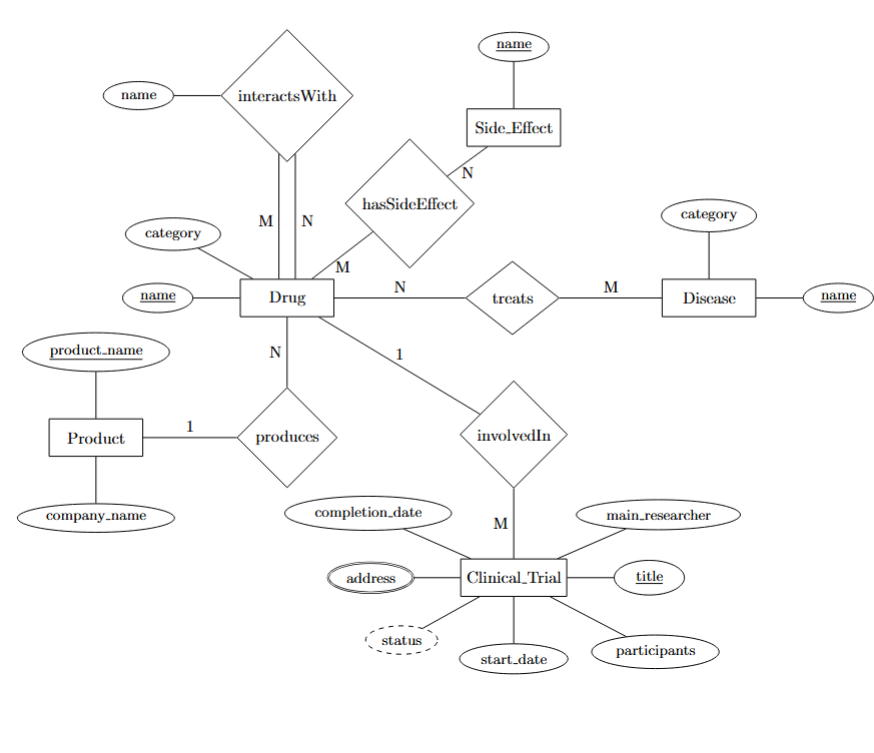
\includegraphics[width=1\textwidth]{er2.png}
    \caption{Revised ER Diagram}
    \label{fig:revised_er_diagram}
\end{figure}

\newpage
\section{Comparison with Original Design}

\begin{enumerate}
    \item Removed all Transitive Dependencies. Separated Product entity from Drug.
    \item All relations now satisfy BCNF requirements.
    \item Explicit foreign key constraints.
    \item Reduced Redundancy.

\end{enumerate}




\end{document}
